\chapter{Aerodynamic application results}


\section{Results}
\label{sec:results}

\subsection[3D Taylor Green vortex: Re 5000]{3D Taylor Green vortex: $Re= 5 \times 10^3$}
\label{sec:3DTGV}

\subsubsection[Cartesian cubic 65x65x65 mesh]{Influence of LES SFS stress model: Cartesian cubic $65 \times 65 \times 65$ mesh} 
\label{sec:TGV3D-Cart65}
The 3D Taylor-Green vortex of $Re= 5 \times 10^3$ case is prepared in the same way described in the Sec. \ref{sec:dampHFModes}. The LES results from the \spaece algorithm simulated in a Cartesian cubic $65 \times 65 \times 65$ mesh and comparison with DNS \cite{dairay2017} is illustrated in Fig. \ref{fig:TGV3D-5k65}. The dynamic k equation LES model dissipates aggressively early on and predicts an over-diffusive KE decay profile (Fig. \ref{fig:TGV3D-5k65-KE}). Nevertheless, as demonstrated earlier in Sec \ref{sec:minimizeArtificialDissipation}, the \spaece algorithm KE decay rate exactly matches with the total dissipation rate (Fig. \ref{fig:TGV3D-5k65-epsilon}). Contribution from the LES sub-filter scale dissipation is higher than the molecular dissipation. 

\begin{figure}[!h]
\centering
\subfloat[KE decay (top) and decay rate (bottom)]{\includegraphics[width=\imgHalfWidth\columnwidth]{TGV3D/Re5000/spaece/65x65x65/3DTGV_Re5000_spaeceFoamCNTGV_dynKEqnHeinz_8x8_k_dkdt.pdf}\label{fig:TGV3D-5k65-KE}}
\subfloat[KE decay rate vs dissipation rate(s)]{\includegraphics[width=\imgHalfWidth\columnwidth]{TGV3D/Re5000/spaece/65x65x65/3DTGV_Re5000_spaeceFoamCNTGV_dynKEqnHeinz_8x8_epsilon0.pdf}\label{fig:TGV3D-5k65-epsilon}} 
\caption{\spaeceA LES results of the 3D Taylor-Green vortex of $Re= 5 \times 10^3$ case with dynamic k equation turbulence model performed in a Cartesian cubic $65 \times 65 \times 65$ mesh} 
\label{fig:TGV3D-5k65}
\end{figure}

In Fig. \ref{fig:TGV3D-5k-3solver65}, KE decay rate and total dissipation rate from the \spaeceA, \spaeceARC and \piso algorithms are compared. Application of Rhie-Chow correction resulted in early dissipation in \spaeceARC and \piso algorithms compared to the \spaeceA algorithm (see Fig. \ref{fig:TGV3D-5k-3solver65-dkdt} at $t/t_c = 5$). Although, the differences in KE decay rate are small, the \piso algorithm has least total-dissipation rate ( i.e. most artificial dissipation) among the three algorithms. 

\begin{figure}[!h]
\centering
\subfloat[KE decay rate $ -\frac{dk}{dt}$]{\includegraphics[width=\imgHalfWidth\columnwidth]{TGV3D/Re5000/pisoVsSpaeceA6VsA6RC/cube/65x65x65/3DTGV_Re5000_dynKEqnHeinz_8x8_dkdt.pdf}\label{fig:TGV3D-5k-3solver65-dkdt}}
\subfloat[Total dissipation rate $\nu_{eff}$]{\includegraphics[width=\imgHalfWidth\columnwidth]{TGV3D/Re5000/pisoVsSpaeceA6VsA6RC/cube/65x65x65/3DTGV_Re5000_dynKEqnHeinz_8x8_nuEff.pdf}\label{fig:TGV3D-5k-3solver65-nuEff}} 
\caption{KE decay rate (left) and total dissipation rate (right) comparison for the 3D Taylor-Green vortex of $Re = 5\times10^3$ case among the \piso, \spaeceA and \spaeceARC algorithms performed in a Cartesian cubic $65 \times 65\times 65$ mesh} 
\label{fig:TGV3D-5k-3solver65}
\end{figure}


\begin{figure}[!h]
\centering
\subfloat[\spaeceARC algorithm]{\includegraphics[width=\imgFortySeven\columnwidth]{TGV3D/Re5000/spaeceFoamCNTGV/A6RC/65cubed/spaeceA6RC_nut_time90.png}\label{fig:TGV3D-5kNut65-spaeceA6RC}}
\subfloat[\piso algorithm]{\includegraphics[width=\imgFiftyThree\columnwidth]{TGV3D/Re5000/pisoFoamMod/65cubed/piso_nut_time90.png}\label{fig:TGV3D-5kNut65-piso}} 
\caption{Eddy viscosity $\nu_t$ comparison for the 3D Taylor-Green vortex of $Re = 5\times10^3$ case between the \spaeceARC and \piso algorithms performed in a Cartesian cubic $65 \times 65\times 65$ mesh} 
\label{fig:TGV3D-5kNut65}
\end{figure}


When compared to the artificial dissipation free \spaeceA algorithm, the Rhie-Chow corrected \spaeceARC algorithm has moderate artificial dissipation present. However, it shows a significant improvement over the \piso algorithm. Fig. \ref{fig:TGV3D-5kNut65} compares the eddy viscosity $\nu_t$ in the $y =0$ cross-section at time $t/t_c = 9$, where the \spaeceARC algorithm shows substantially higher eddy viscosity $\nu_t$ values compared to the \piso algorithm.

%\clearpage
%\newpage

%\line(x-slope,y-slope){length}
%\line(1,0){300}

%\rule{length}{thickness}
%\rule{\paperwidth}{1pt}
%\rule{\textwidth}{1pt}

\subsubsection[Cartesian cubic 129x129x129 mesh:]{Influence of mesh refinement: Cartesian cubic $129 \times 129 \times 129$ mesh} 
\label{sec:TGV3D-Cart129}
Following the previous section, the 3D Taylor-Green vortex is simulated in refined Cartesian cubic $129 \times 129 \times 129$ mesh. Compared to the coarse mesh, LES on the refined mesh resolves more scales, thus have less SFS stress (Fig \ref{fig:TGV3D-5k129-epsilon}). The effect early aggressive dissipation by the dynamic SFS model is reduced albeit present! This signifies importance of accurate SFS scale model in DNS. Similar to the coarse mesh, the \spaeceARC algorithm has substantially less artificially dissipation (Fig \ref{fig:TGV3D-5k-3solver-129}) and higher eddy viscosity $\nu_t$ values (Fig. \ref{TGV3D-5kNut129}) compared to the \piso algorithm. 

\begin{figure}[!h]
\centering
\subfloat[KE decay (top) and decay rate (bottom)]{\includegraphics[width=\imgHalfWidth\columnwidth]{TGV3D/Re5000/spaece/129x129x129/3DTGV_Re5000_spaeceFoamCNTGV_dynKEqnHeinz_8x8_k_dkdt.pdf}\label{fig:TGV3D-5k129-KE}}
\subfloat[KE decay rate vs dissipation rate(s)]{\includegraphics[width=\imgHalfWidth\columnwidth]{TGV3D/Re5000/spaece/129x129x129/3DTGV_Re5000_spaeceFoamCNTGV_dynKEqnHeinz_8x8_epsilon0.pdf}\label{fig:TGV3D-5k129-epsilon}} 
\caption{\spaeceA LES results of the 3D Taylor-Green vortex of $Re= 5 \times 10^3$ case with dynamic k equation turbulence model performed in a Cartesian cubic $129 \times 129 \times 129$ mesh} 
\label{fig:TGV3D-5k129}
\end{figure}



\begin{figure}[!h]
\centering
\subfloat[KE decay rate $ -\frac{dk}{dt}$]{\includegraphics[width=\imgHalfWidth\columnwidth]{TGV3D/Re5000/pisoVsSpaeceA6VsA6RC/cube/129x129x129/3DTGV_Re5000_dynKEqnHeinz_8x8_dkdt.pdf}\label{fig:TGV3D-5k-3solver-129-dkdt}}
\subfloat[Total dissipation rate $\nu_{eff}$]{\includegraphics[width=\imgHalfWidth\columnwidth]{TGV3D/Re5000/pisoVsSpaeceA6VsA6RC/cube/129x129x129/3DTGV_Re5000_dynKEqnHeinz_8x8_nuEff.pdf}\label{fig:TGV3D-5k-3solver-129-nuEff}} 
\caption{KE decay rate (left) and total dissipation rate (right) comparison among the \piso, \spaeceA and \spaeceARC algorithms performed in a Cartesian cubic $129 \times 129 \times 129$ mesh} 
\label{fig:TGV3D-5k-3solver-129}
\end{figure}


\begin{figure}[!h]
\centering
\subfloat[\spaeceARC algorithm]{\includegraphics[width=\imgFortySeven\columnwidth]{TGV3D/Re5000/spaeceFoamCNTGV/A6RC/129cubed/spaeceA6RC_nut_time90}\label{fig:TGV3D-5kNut129-spaeceA6RC}}
\subfloat[\piso algorithm]{\includegraphics[width=\imgFiftyThree\columnwidth]{TGV3D/Re5000/pisoFoamMod/129cubed/piso_nut_time90}\label{fig:TGV3D-5kNut129-piso}} 
\caption{Eddy viscosity $\nu_t$ comparison for the 3D Taylor-Green vortex of $Re = 5\times10^3$ case between the \spaeceARC and \piso algorithms performed in a Cartesian cubic $129 \times 129 \times 129$ mesh} 
\label{fig:TGV3D-5kNut129}
\end{figure}





\clearpage
\subsubsection[Right-angle triangulated prismatic (65x65)x2x65 mesh]{Influence of non-orthogonality: Right-angle triangulated prismatic $(65 \times 65) \times 2 \times 65$ mesh}
\label{sec:TGV3D-prism}
Each control volume of the Cartesian cubic $65 \times 65 \times 65$ mesh is split diagonally in $z$ normal plane to convert the cube into two right-angle prism, resulting in a $(65 \times 65) \times 2 \times 65$ mesh. The prism has three orthogonal and two non-orthogonal faces. Similar to the Cartesian cubic meshes (Sec. \ref{sec:TGV3D-Cart65} and \ref{sec:TGV3D-Cart129}), the \spaeceA algorithm doesn't introduce and non-physical dissipation (Fig. \ref{fig:TGV3D-5kPrism-3solver65-dkdt}) and the \spaeceARC algorithm has higher total-dissipation rate compared to the \piso algorithm (Fig. \ref{fig:TGV3D-5kPrism-3solver65-nuEff}).     

\begin{figure}[!h]
\centering
\subfloat[KE decay rate $ -\frac{dk}{dt}$]{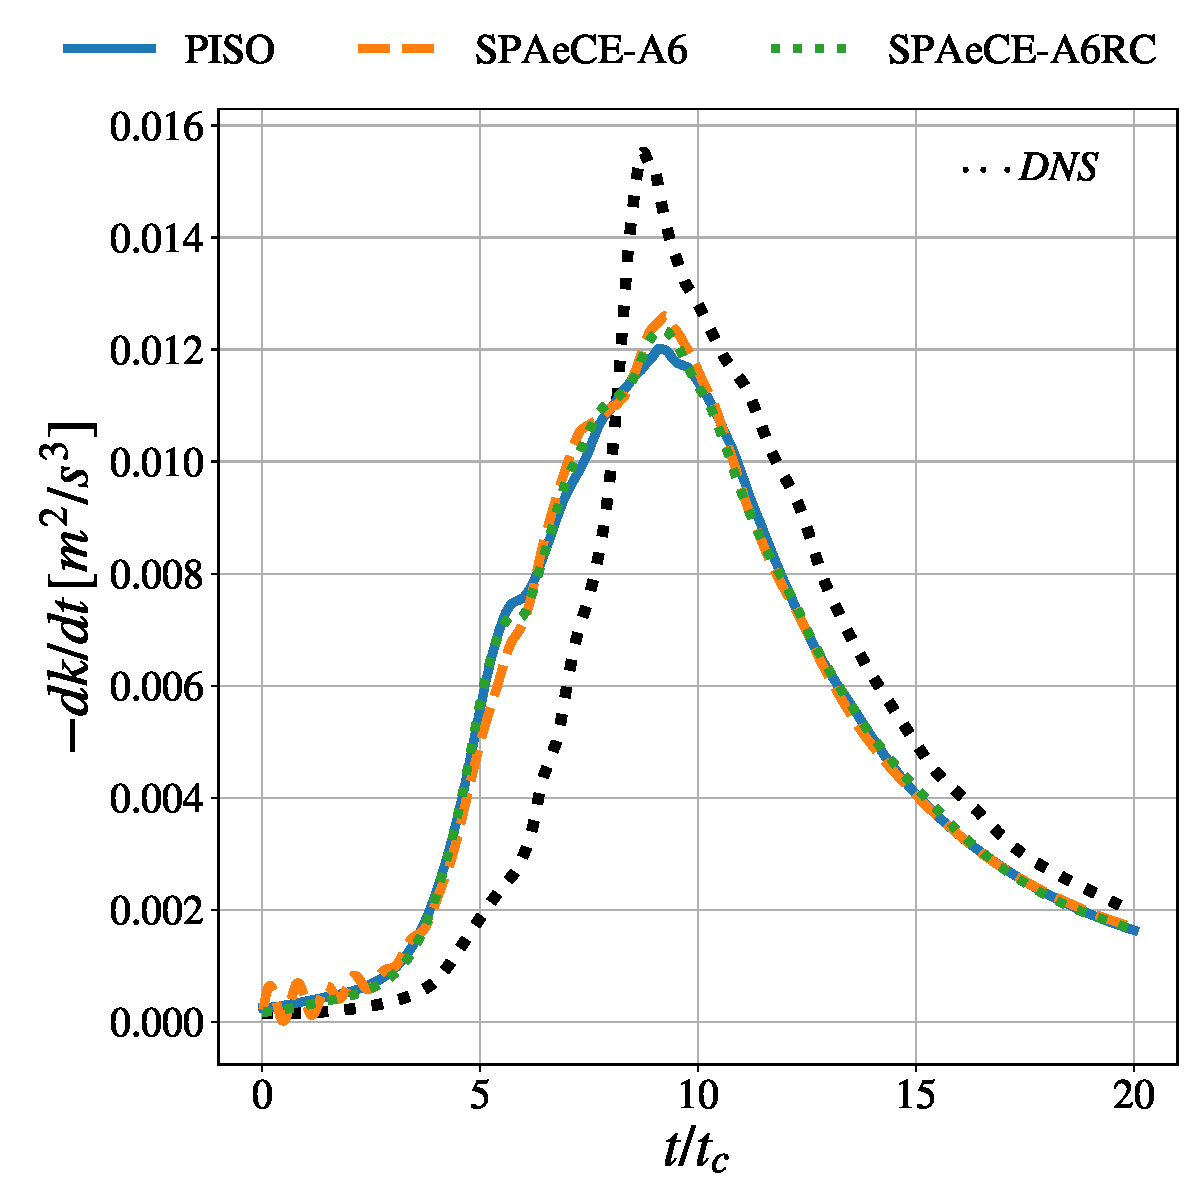
\includegraphics[width=\imgHalfWidth\columnwidth]{TGV3D/Re5000/pisoVsSpaeceA6VsA6RC/prism/65x65x65/3DTGV_unstructured_uniformRightAnglePrism_Re5000_dynKEqnHeinz_8x8_dkdt.pdf}\label{fig:TGV3D-5kPrism-3solver65-dkdt}}
\subfloat[Total dissipation rate $\nu_{eff}$]{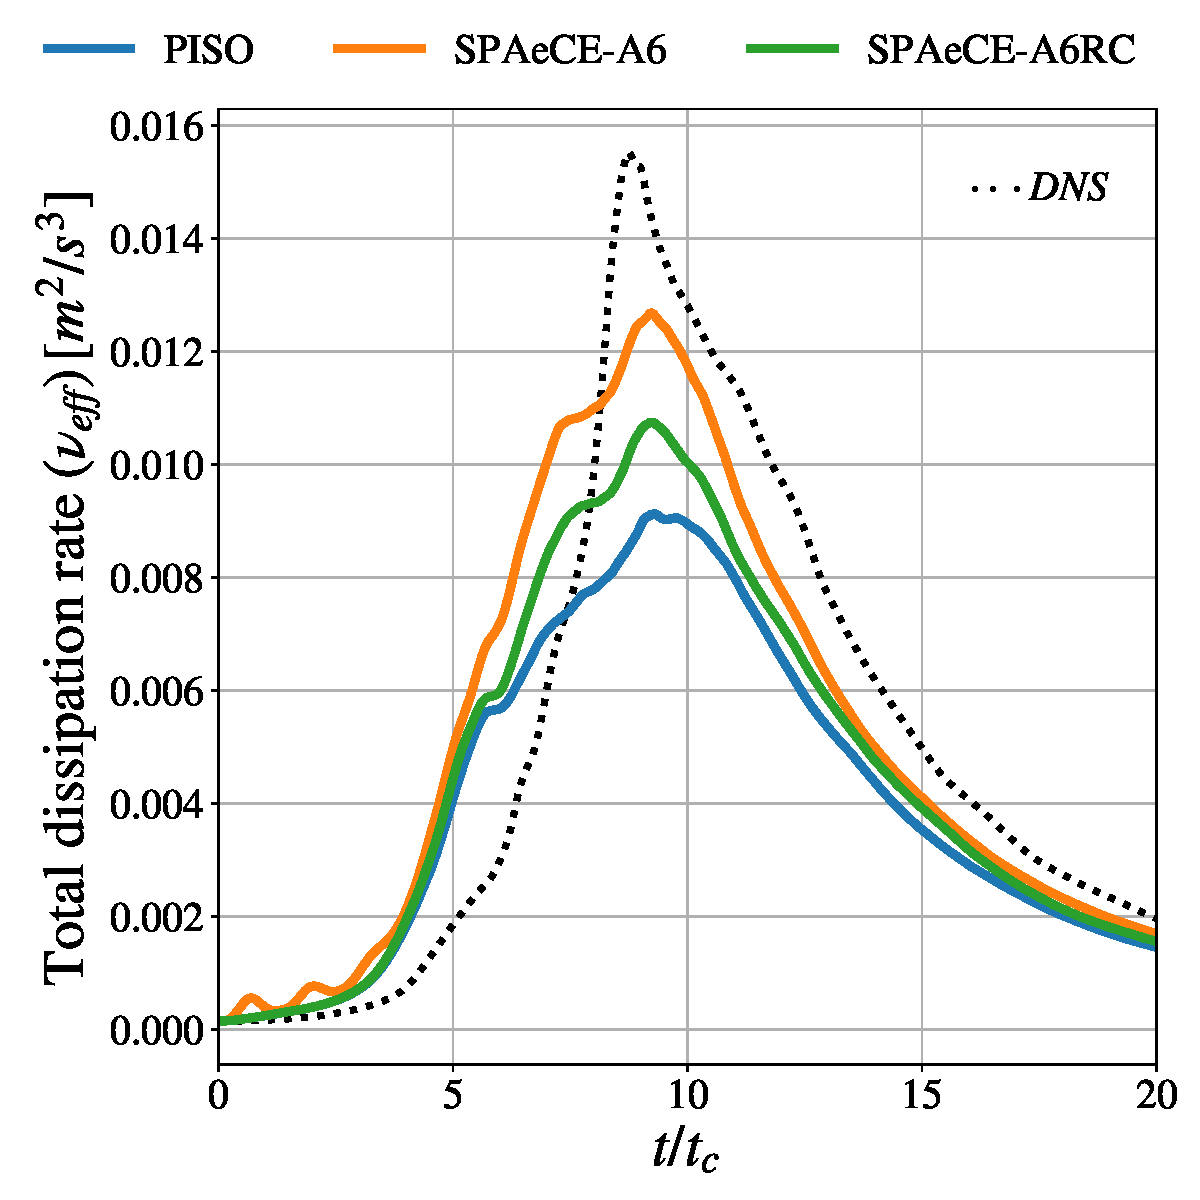
\includegraphics[width=\imgHalfWidth\columnwidth]{TGV3D/Re5000/pisoVsSpaeceA6VsA6RC/prism/65x65x65/3DTGV_unstructured_uniformRightAnglePrism_Re5000_dynKEqnHeinz_8x8_nuEff.pdf}\label{fig:TGV3D-5kPrism-3solver65-nuEff}} 
\caption{KE decay rate (left) and total dissipation rate (right) comparison for the 3D Taylor-Green vortex of $Re = 5\times10^3$ case among the \piso, \spaeceA and \spaeceARC algorithms performed in a right-angle triangulated prismatic $(65 \times 65) \times 2 \times 65$ mesh} 
\label{fig:TGV3D-5kPrism-3solver65}
\end{figure}

\subsubsection{Influence of non-uniform mesh}
\label{sec:TGV3D-nonUniform}

In Fig. \ref{fig:TGV3D-inv-hex}, we have shown the importance of using the mid-point interpolation scheme instead of a linear scheme for KE conservation in a non-uniform Cartesian hexagonal $65 \times 65 \times 65$ mesh. However, the mid-point interpolation in a non-uniform mesh provides less than 2nd order accuracy thus influence the overall results. Fig. \ref{fig:3DTGV-5k-CubeHex} compares the 3D Taylor-Green vortex of $Re = 5\times10^3$ results between the cubic and hexagonal mesh. Although both meshes are Cartesian and have the same cell count, the non-uniform hexagonal mesh is slightly more dissipative and less accurate compared to corresponding uniform, cubic mesh. Thus with mid-point interpolation, accuracy is traded off for KE conservation and stability.

\begin{figure}[!h]
\centering
\subfloat[KE decay (top) and decay rate (bottom)]{\includegraphics[width=\imgHalfWidth\columnwidth]{TGV3D/Re5000/cubeVsHex/65x65x65/3DTGV_Re5000_spaeceFoamCNTGV_dynKEqnHeinz_8x8_k_dkdt.pdf}\label{fig:label one}}
\subfloat[KE decay rate vs dissipation rate(s)]{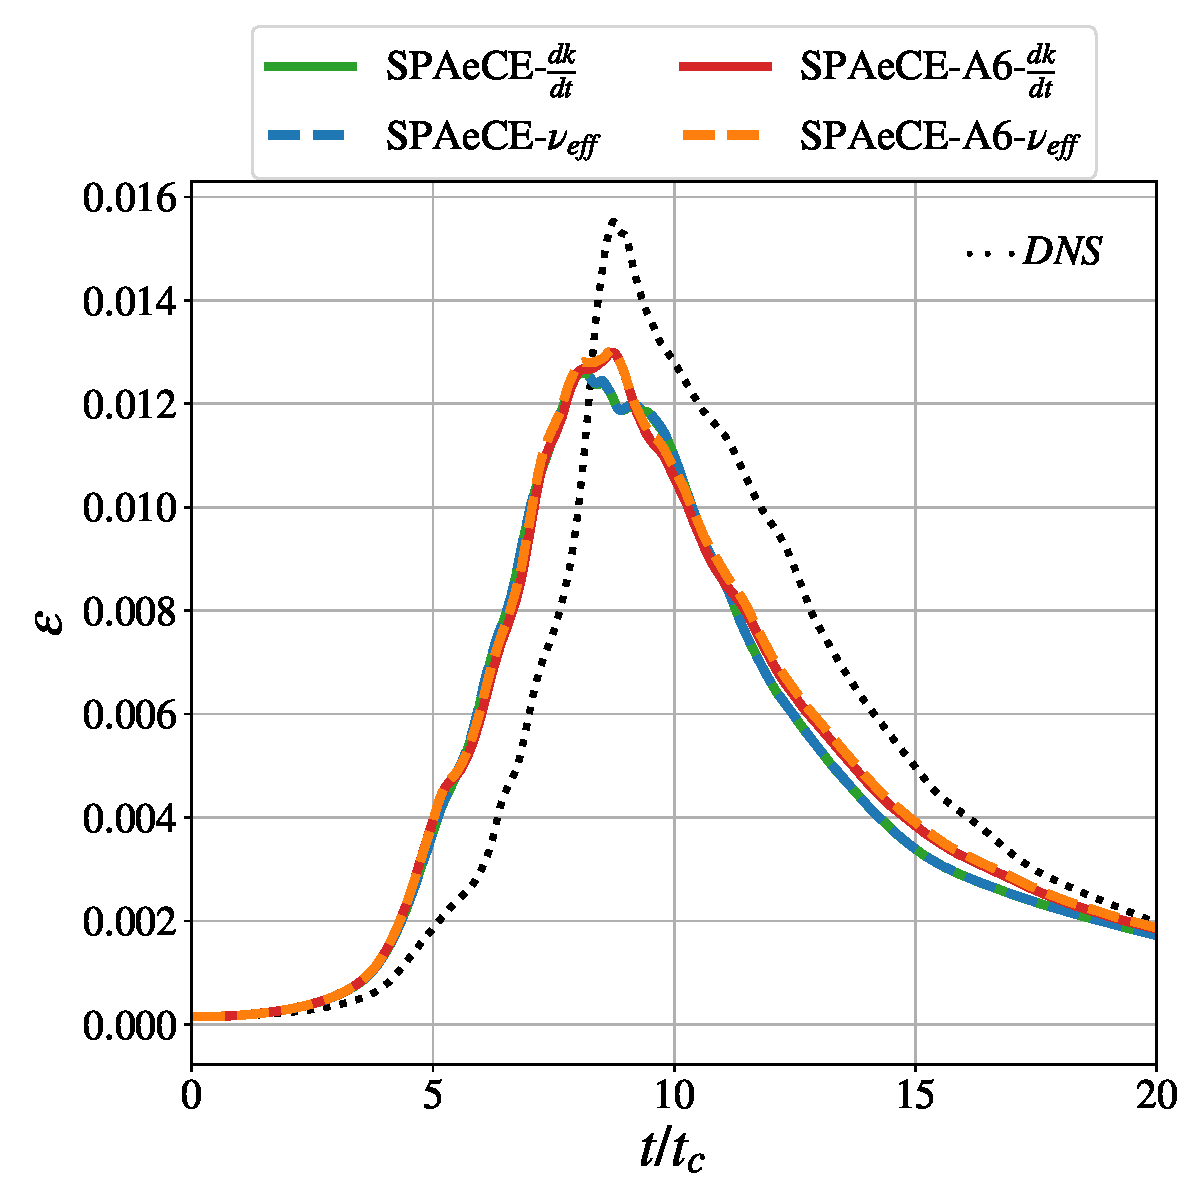
\includegraphics[width=\imgHalfWidth\columnwidth]{TGV3D/Re5000/cubeVsHex/65x65x65/3DTGV_Re5000_spaeceFoamCNTGV_dynKEqnHeinz_8x8_epsDkdt0.pdf}\label{fig:3DTGV-5k-CubeHex-dissp}} 
\caption{\spaeceA LES results of the 3D Taylor-Green vortex of $Re= 5 \times 10^3$ case with dynamic k equation turbulence model compared between a Cartesian uniform-cubic mesh and a Cartesian non-uniform hexagonal mesh (max. aspect ratio $5.3$) of $65 \times 65 \times 65$ cells} 
\label{fig:3DTGV-5k-CubeHex}
\end{figure}










\clearpage
\subsection[Fully developed channel flow at Re_tau 590]{Fully developed channel flow at $Re_\tau = 590$}
\label{sec:channel590}

Fully developed turbulent flow though a plane channel at Reynolds number based on friction velocity $Re_\tau = 590$ is investigated.
A 3D computational domain formed for channel dimension $(L \times W \times H): 2\pi \times \pi \times 2$. A Cartesian hexagonal $129 \times 129 \times 129$ mesh is used, which is symmetric at the channel boundary layer height $y=1$. The mesh resolution is uniform in the stream-wise and cross-stream direction, and in wall-normal direction, gradually stretched from next-to-wall resolution $y^+ \leqslant 0.5$ (cell center height of the wall adjacent control volumes). The normalized resolution in the stream-wise direction is $x^+ \leqslant 30$ and cross-stream direction is $z^+ \leqslant 15$. The maximum cell aspect ratio at near-wall cells is $\approx 32$ gradually decreased to $1$ at the boundary layer height.

Periodic boundary condition is applied in the stream-wise and cross-stream directions, and no-slip boundary velocity and zero-gradient pressure is applied at channel walls. A time-varying, uniform driving pressure gradient included as a source term in the momentum conservation equation to maintain mean flow rate across the channel constant. LES is performed for three different algorithms \piso, \spaece and \spaeceARC and the dynamic k equation model of Heinz et al. is utilized as the sub-filter-stress model. The regularization and LES filter are defined same as in the 3D ataylor-Green vortex case (Sec. \ref{sec:3DTGV}).

\begin{figure}[!h]
\centering
\subfloat[Mean streamwise velocity]{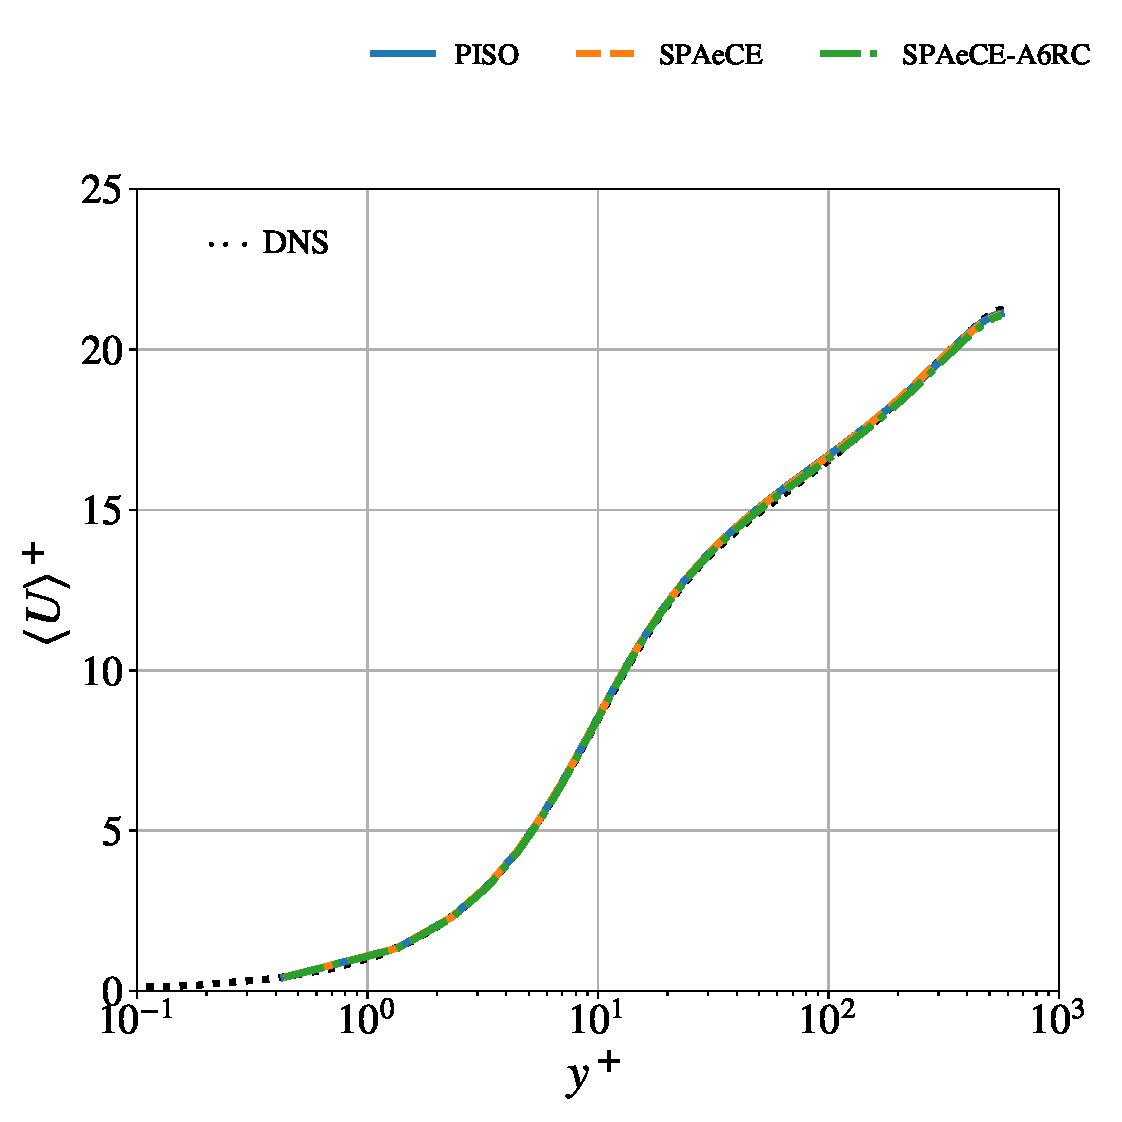
\includegraphics[width=\imgHalfWidth\columnwidth]{channel590/129x129x129/plots/PISOvsSPAeCEvsA6RC/ChannelFlowRe590_cyclic_dynKEqnHeinz_129x129x129-Uf-log.pdf}\label{fig:channel590-Cart129-MeanStreamwiseVelocity}}
\subfloat[Mean shear stress]{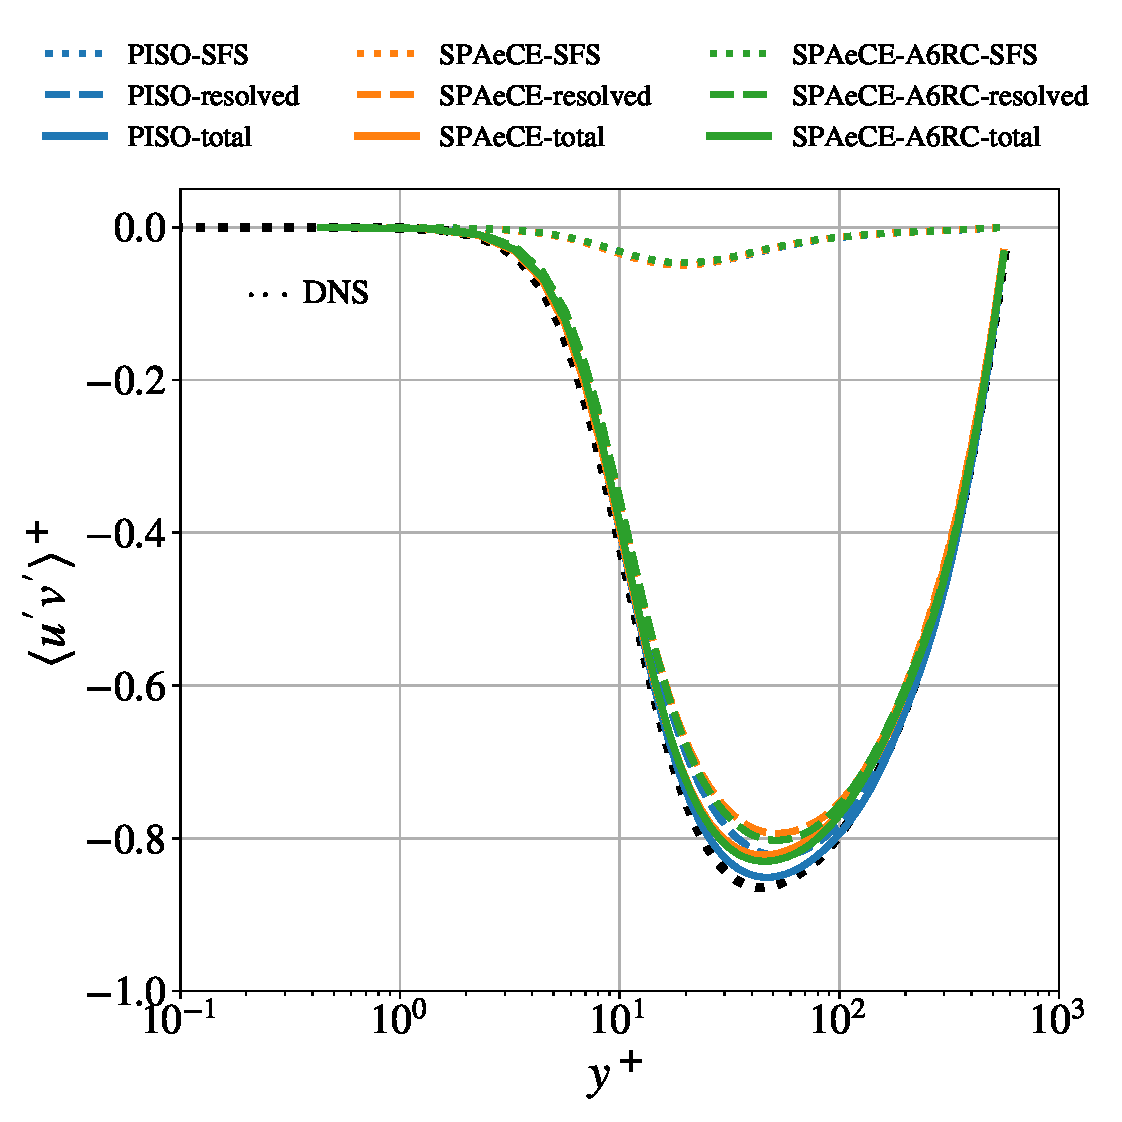
\includegraphics[width=\imgHalfWidth\columnwidth]{channel590/129x129x129/plots/PISOvsSPAeCEvsA6RC/ChannelFlowRe590_cyclic_dynKEqnHeinz_129x129x129-uv-log.pdf}\label{fig:channel590-Cart129-MeanShearStress}} 
\caption{Mean stream-wise velocity and shear stress comparison among the \piso, \spaece and \spaeceARC algorithms in a fully developed channel flow at $Re_\tau = 590$ simulated in a Cartesian hexagonal $129 \times 129 \times 129$ mesh} 
\label{fig:channel590-Cart129}
\end{figure}


The mean streamwise velocity and shear stress comparison is illustrated in Fig. \ref{fig:channel590-Cart129} and compared with DNS profiles derived by Moser et al. \cite{moser1999}. The flow is initialized from a 2D RANS simulation and random perturbation is introduced to facilitate transition to 3D flow. After initial transient time of $200s$, flow statistics is gathered for $300s$. The time-averaged fields are averaged in the homogeneous stream-wise and cross-stream directions. To leverage the symmetry of the fully developed flow, the symmetric profiles averaged again. 

All three algorithms produced an exact match with DNS mean stream-wise velocity profile. The well-refined mesh results in small sub-filter-scale (SFS) stress contribution in the viscous wall region $( y^+ < 50)$ and the resolved stress is overwhelmingly large signifying the simulation transition from LES at the near-wall region $( y^+ < 100)$ to DNS at the channel center $( y^+ > 100)$.

\begin{figure}[!h]
\centering
\subfloat[$y^{+} = 5$]{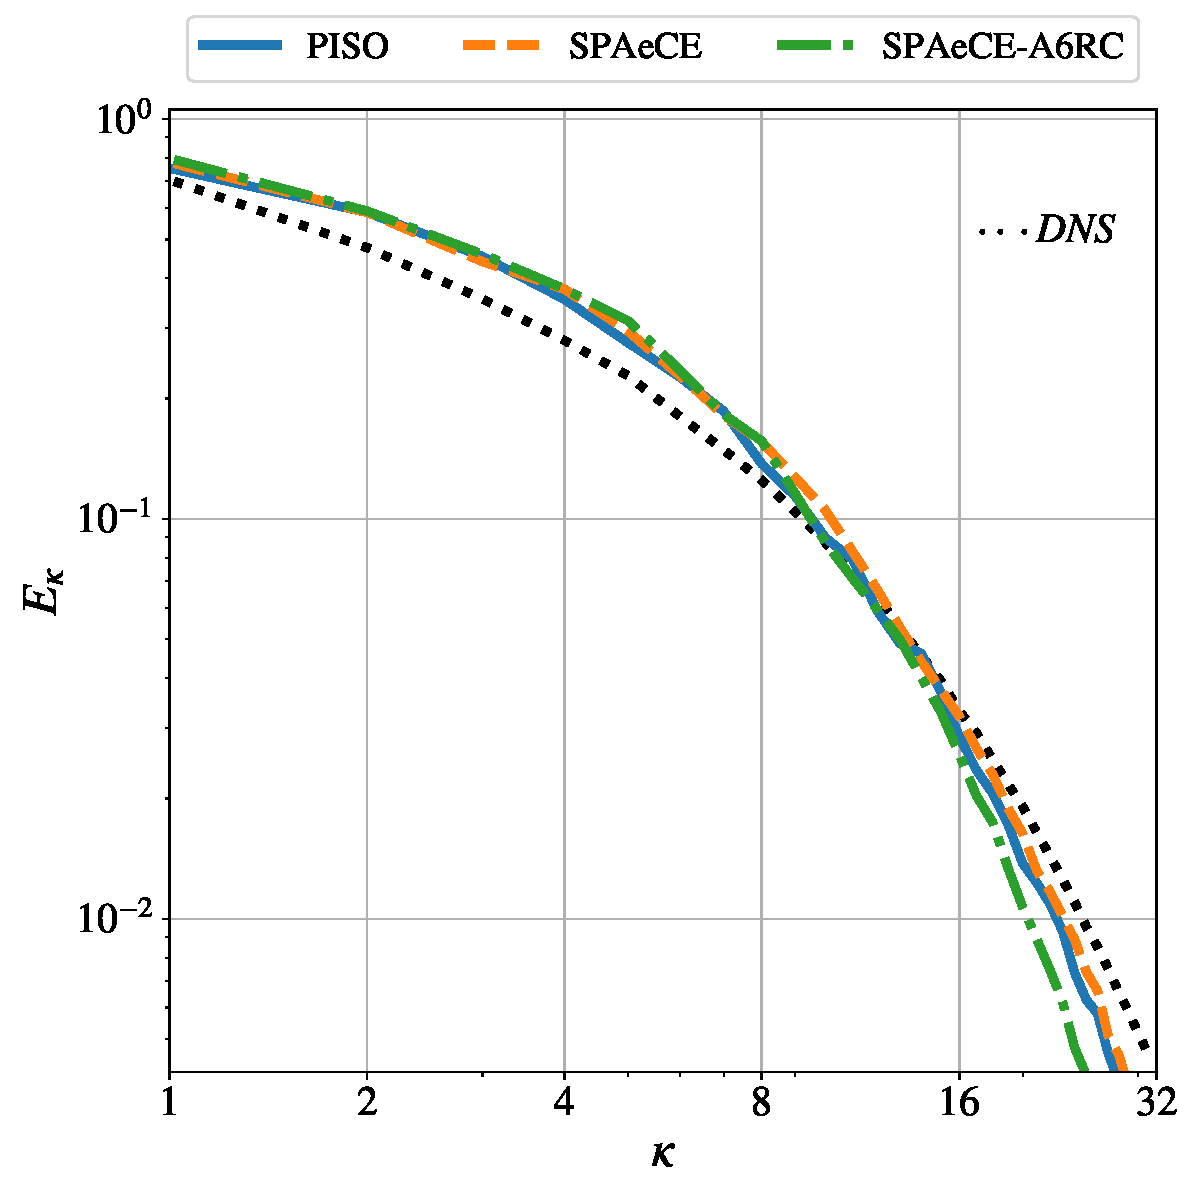
\includegraphics[width=\imgHalfWidth\columnwidth]{channel590/129x129x129/plots/specturmX/specturmX_Y5.pdf}\label{fig:channel590-Cart129-Spec5}}
\subfloat[$y^{+} = 587$]{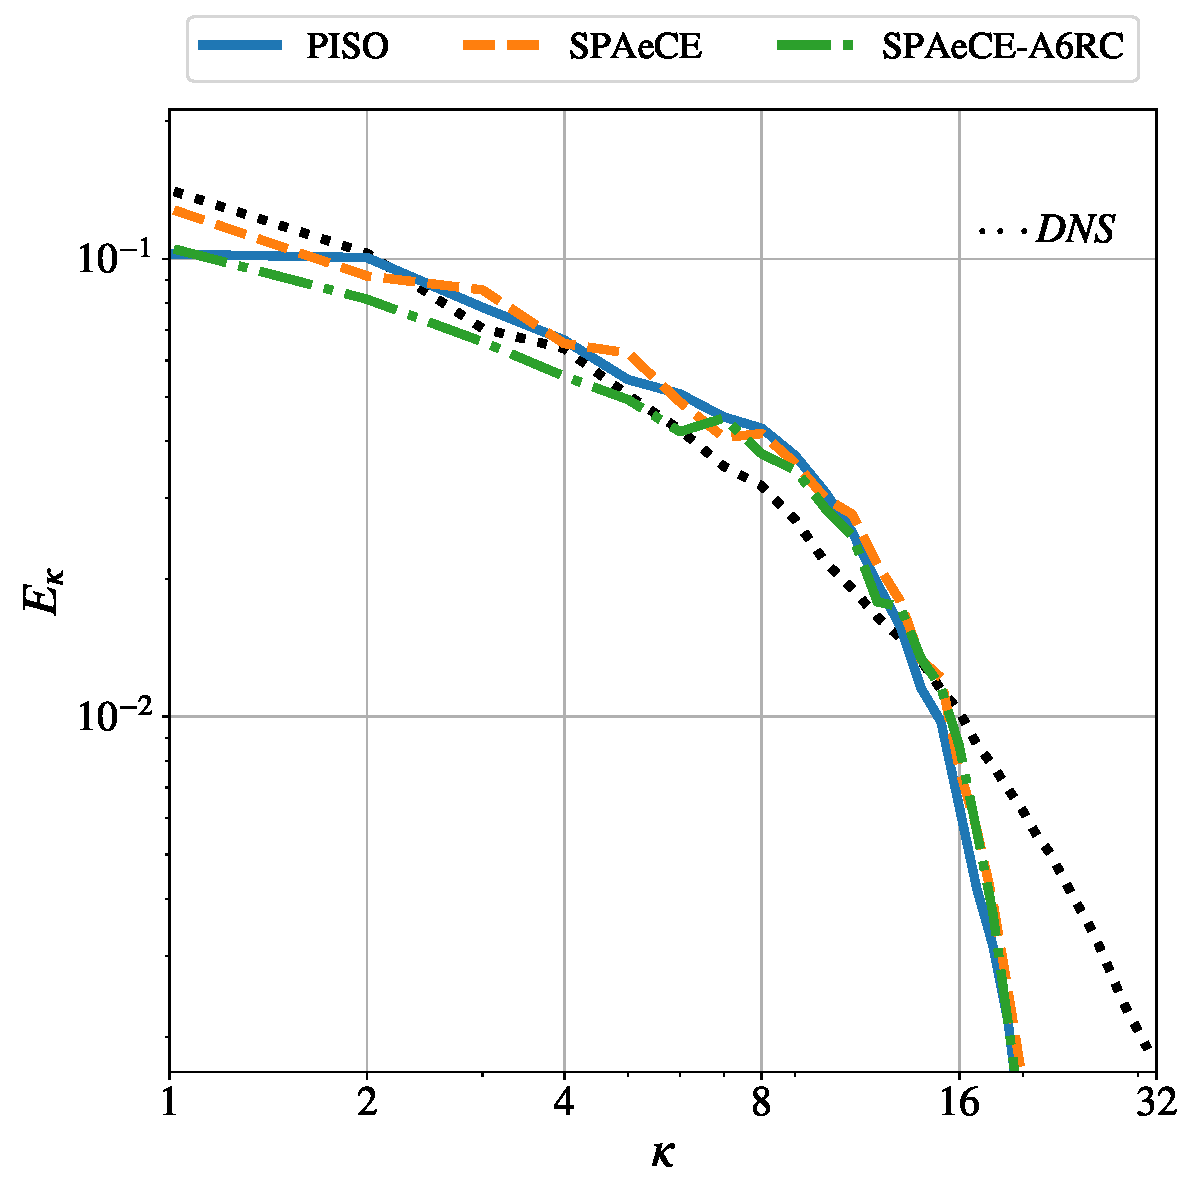
\includegraphics[width=\imgHalfWidth\columnwidth]{channel590/129x129x129/plots/specturmX/specturmX_Y587.pdf}\label{fig:channel590-Cart129-Spec587}} 
\caption{KE spectrum comparison in stream-wise direction at wall-normal heights $y^+ = 5, 587$ compared among the \piso, \spaece and \spaeceARC algorithms in a fully developed channel flow at $Re_\tau = 590$ simulated in a Cartesian hexagonal $129 \times 129 \times 129$ mesh} 
\label{fig:channel590-Cart129-Spec}
\end{figure}

KE spectrum in stream-wise direction at two wall-normal heights $y^+ = 5, \, 587$ are compared in Fig. \ref{fig:channel590-Cart129-Spec}. All three algorithms are in good agreements wit the DNS profile. KE is over predicted in low wave numbers and under-predicted in higher wave numbers. 


\subsubsection{Fully developed channel flow: wall-modeled}


\newpage
\textbf{To do list}
\begin{enumerate}
\item Once the regularization approach is finalized, compare performance among \piso, \spaece and \spaeceARC algorithms.

\item Investigate if there is any benefit of \textit{consistent} approach in Poisson pressure correction (lots of testing and validation).

\item Fully developed channel flow in unstructured grid: shall I make a hybrid grid with Cartesian cell near wall and Delauney triangulation at he core? Or a lower Reynolds number case while limiting $x^+ < 5$ to control non orthogonality?

\item Complete the wall modeled case. Review how the results vary for unstructured, non-orthogonal mesh.

   

\end{enumerate}